\subsection{Методика построения трехмерной модели исследуемого устройства}

Создание модели печатной платы было начато в САПР \textit{Altium Designer}.
В нём была создана библиотека УГО принципиальная схема устройства.
Затем, по логике создания моделей в САПР печатных плат подобных \textit{Altium Designer} должны были быть созданы библиотеки посадочных мест, соедиение их с УГО размещенных на принципиальной схеме.
После чего надо было бы разнести посадочные места на печатной плате и произвести трассировку.

Однако я поступил не так.
Из-за своего изначального предпочтения к использовонию программ с открытым исходным кодом было принято решение использовать САПР печатных плат \textit{KiCAD}.

В тот момент процедура создания печатных плат в \textit{KiCAD}, казалась проще, чем в \textit{Alitum Designer}. Всё дело в том, что у \textit{KiCAD} существует своя библиотека посадочных мест с трёхмерными моделями соотвествующих компонентов в формате \textit{STEP} и \textit{WRL}. Также на \textit{Github} была найдена готовая библиотека УГО соотвествующая ГОСТ.
В \textit{KiCAD} нет предустановленного встроенного автотрассировщика и потому разводка платы производилась вручную,
несмотря на то что можно было бы установить автотрассировщик \textit{freerouting}.

На этом этапе казалось, что выбор \textit{KiCAD} в качестве САПР печатных плат всё только упрощает, поскольку теперь было достаточно:
\begin{enumerate}[label={\arabic*.}]
\item Создать схему электрическую принципиальную, используя готовую библиотеку УГО.
\item На схеме установить соотвествие между УГО и посадочными местами, у которых есть свои трёхмерные модели.
\item Импортировать получившиеся связи непосредственно в документ, в котором осуществляется разводка печатной платы.
\item Рапределить компоненты в группы и провести дорожки наиболее эффективных способом.
\end{enumerate}

Это и было сделано. На тот момент подозрений о том, что это приведёт к каким-либо проблемам не было.

\begin{figure}[H]
  \centering
  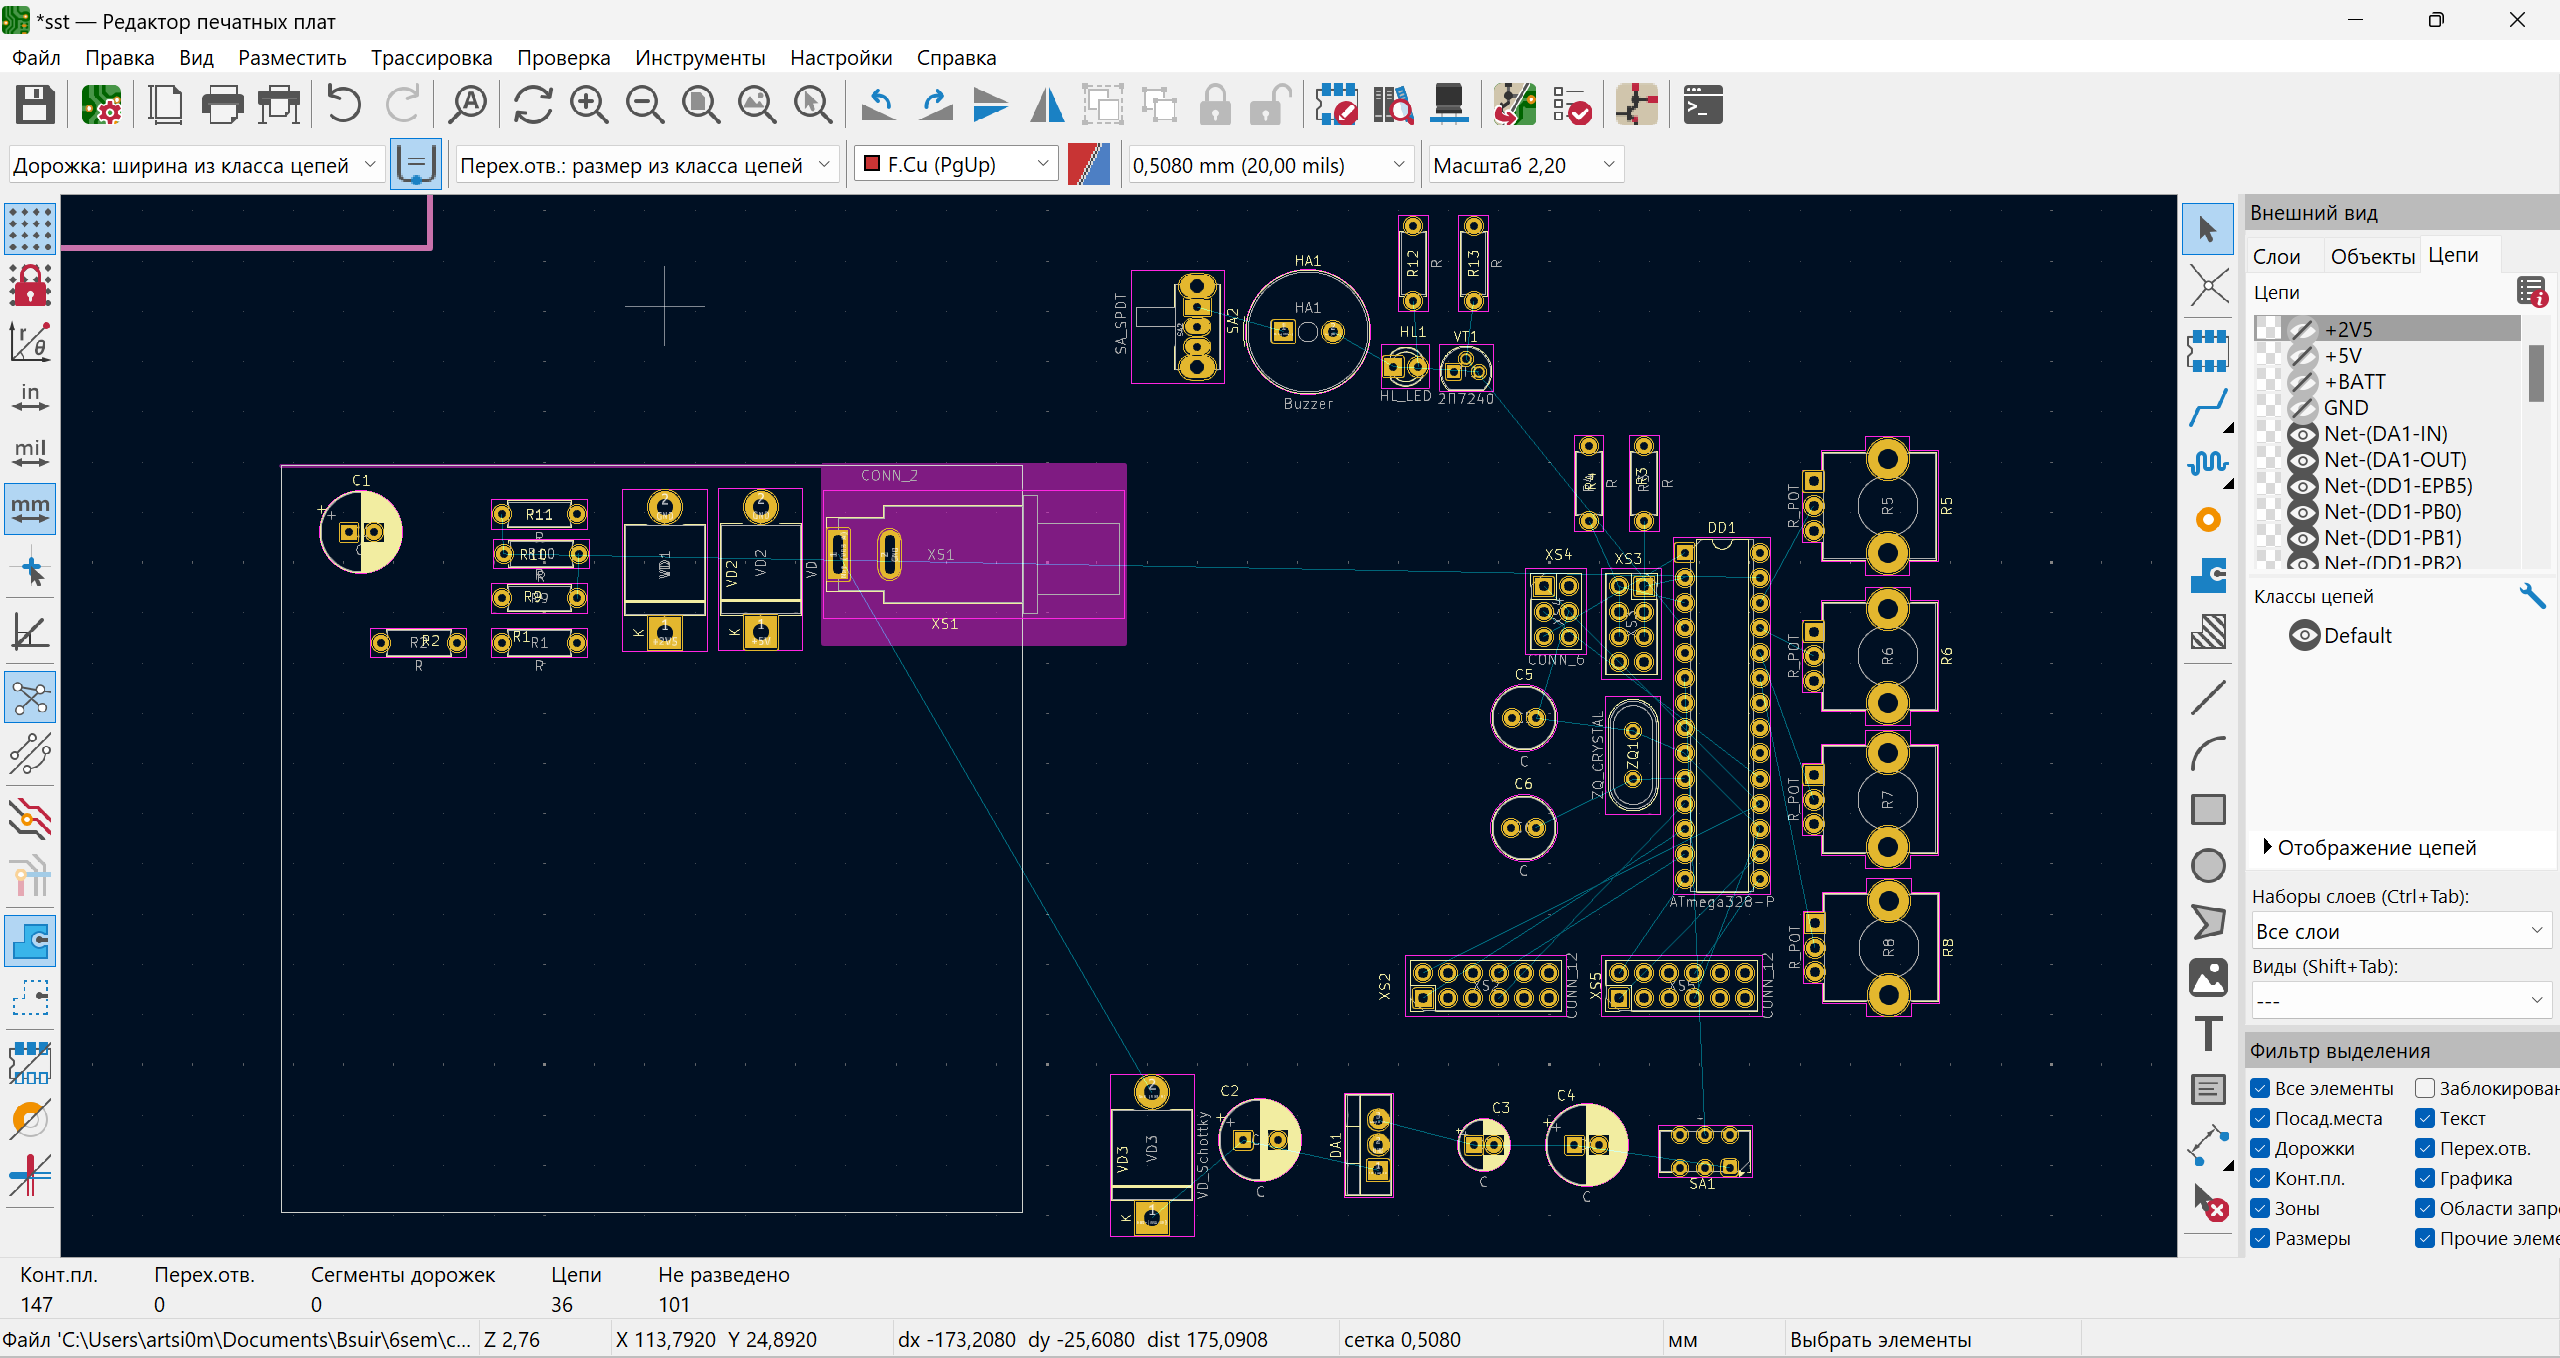
\includegraphics[scale = 0.20]{../img/scrot/Screenshot-2024-05-02-173914.png}
 \caption{Скриншот окна САПР \textit{KiCAD} в котором скрыты цепи относящиеся к питанию и компоненты распределены по группам.}
\end{figure}

Была произведена разводка первой печатной платы:
сначала скрыты цепи связанные с питанием, затем компоненты были объеденены в группы, после чего расставлены по контуру печатной платы и соедены дорожками.

Чтобы заново не производить разводку, а если быть предельно точным,
соединение компонентов было сделать две последующие компоновки печатной платы следующим способом:


В случае второй компоновки просто заменить расположение некоторых посадочных мест, таким образом, чтобы они оказались на другой стороне печатной платы, но подали в нужные отверстия печатной платы. В основном это относилось к резисторам, которые в последствии были использованы, как элементы выделяющие тепло в термическом анализе.


В случае третьей платы были заменены некоторые посадочные места, на минитюаризированные аналоги, в описании которых при этом значился тот же самый шаг (\textit{pitch}) между отверстиями.

\begin{figure}[H]
  \centering
  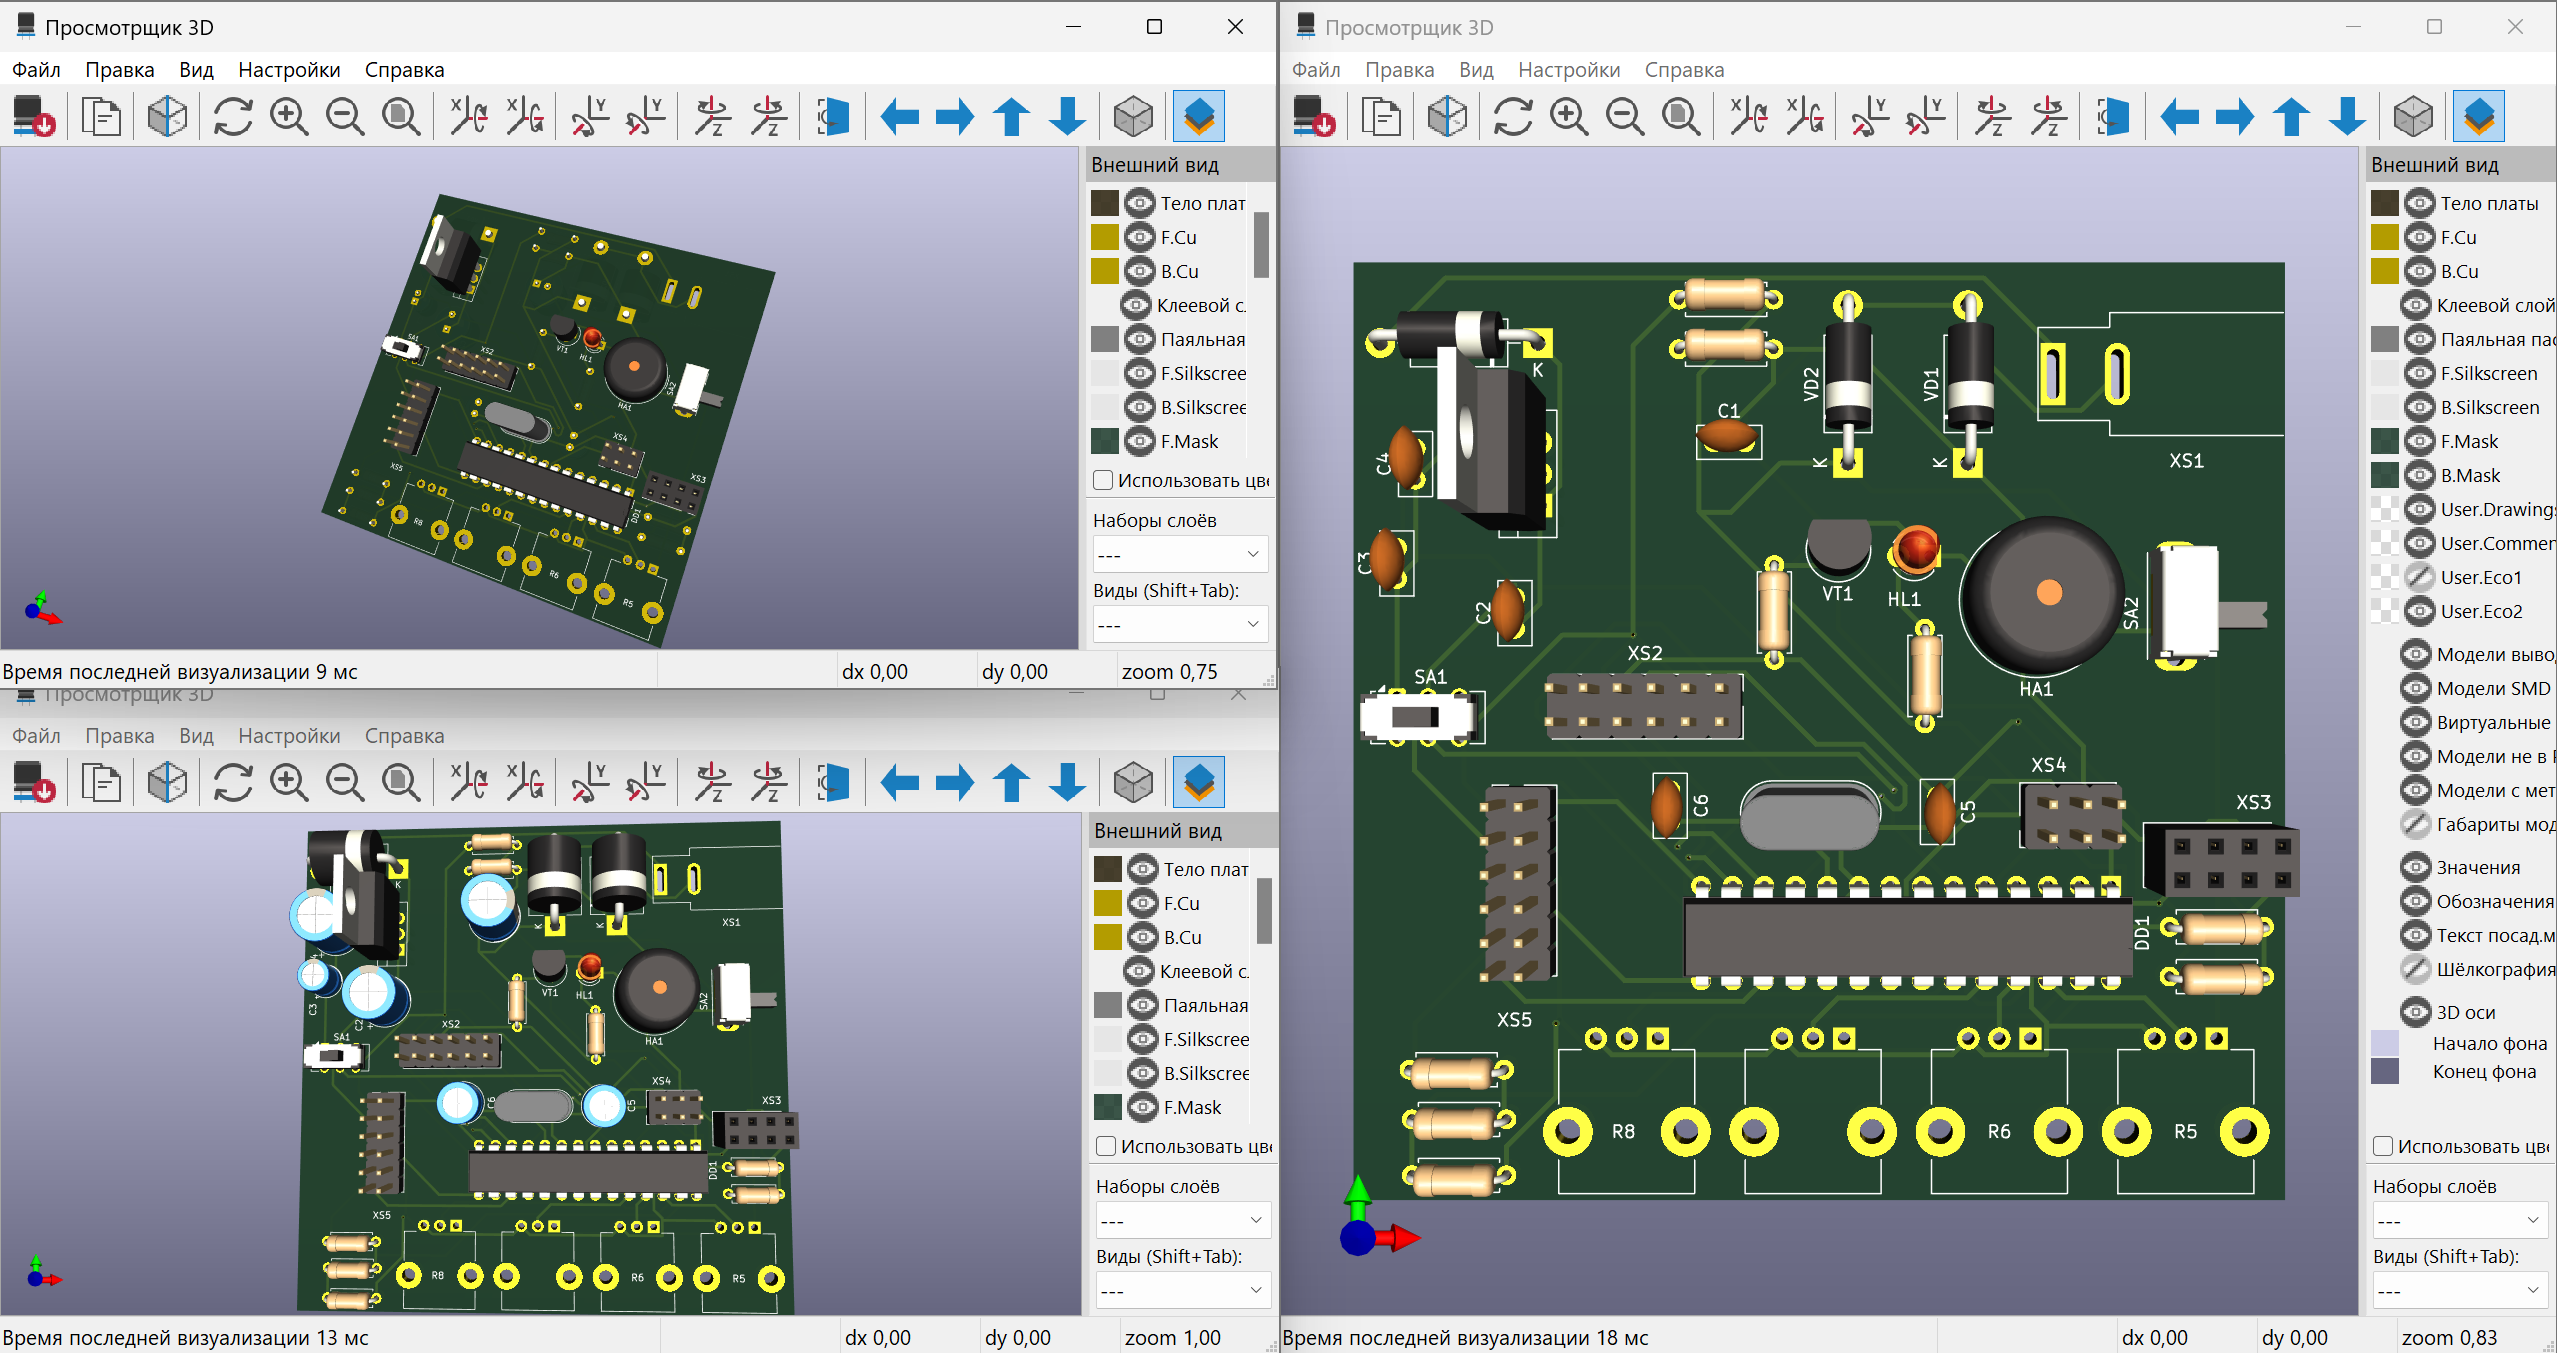
\includegraphics[scale = 0.20]{../img/scrot/Screenshot-2024-05-07-112847.png}
 \caption{Скриншот окон просмотрщика трёхмерных моделей САПР \textit{KiCAD}}
\end{figure}


Полученные варианты печатной платы необходимо экспортировать в \textit{SOLIDWORKS} для проведения дальньшей симуляции. И вот здесь возникли проблемы с получившийся моделью.

\begin{figure}[H]
  \centering
  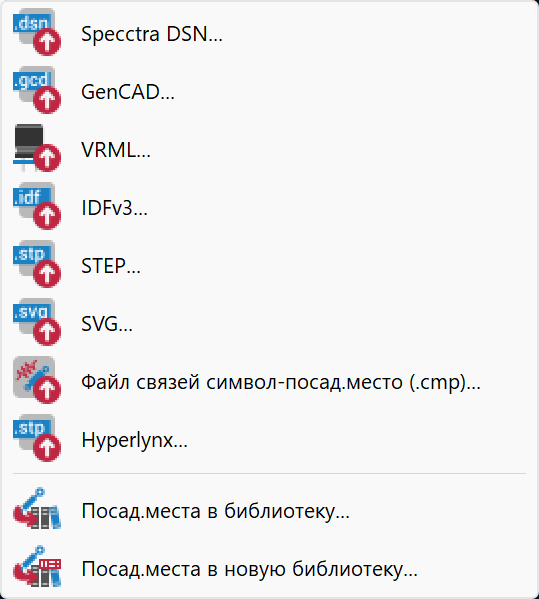
\includegraphics[scale = 0.4]{../img/scrot/Screenshot-2024-05-06-191242.png}
  \caption{Скриншот меню экспорта печатной платы в САПР \textit{KiCAD} }
\end{figure}

В первую очередь была осуществлена попытка экспортировать печатную плату из \textit{KiCAD} в формате \textit{STEP}. Конечно же модель успешно экспортировалась. Проблема была в другом: полученная модель была излишне подробна. Расчет такой модели в \textit{SOLIDWORKS Simulation} мог занимать по пять минут для частотного анализа, но, что более критично, часто приводил к зависанию или падению \textit{SOLIDWORKS}.

Для того, чтобы решить эту проблему было предпринята попытка экспортировать в формате \textit{IDFv3}. Это решение было принято из-за того, что подразумевалось,
что при импорте полученного \textit{IDF} файла в \textit{SOLIDWORKS} будет автоматически использовано дополнение \textit{Circuit WORKS}, которое в случае импорта из \textit{Аltium Designer} упрощало модель таким образом, что вместо точных трехмерных моделей компонентов получались схожие, но значительно упрощенные трёхмерные геометрические фигуры.


\begin{figure}[H]
  \centering
  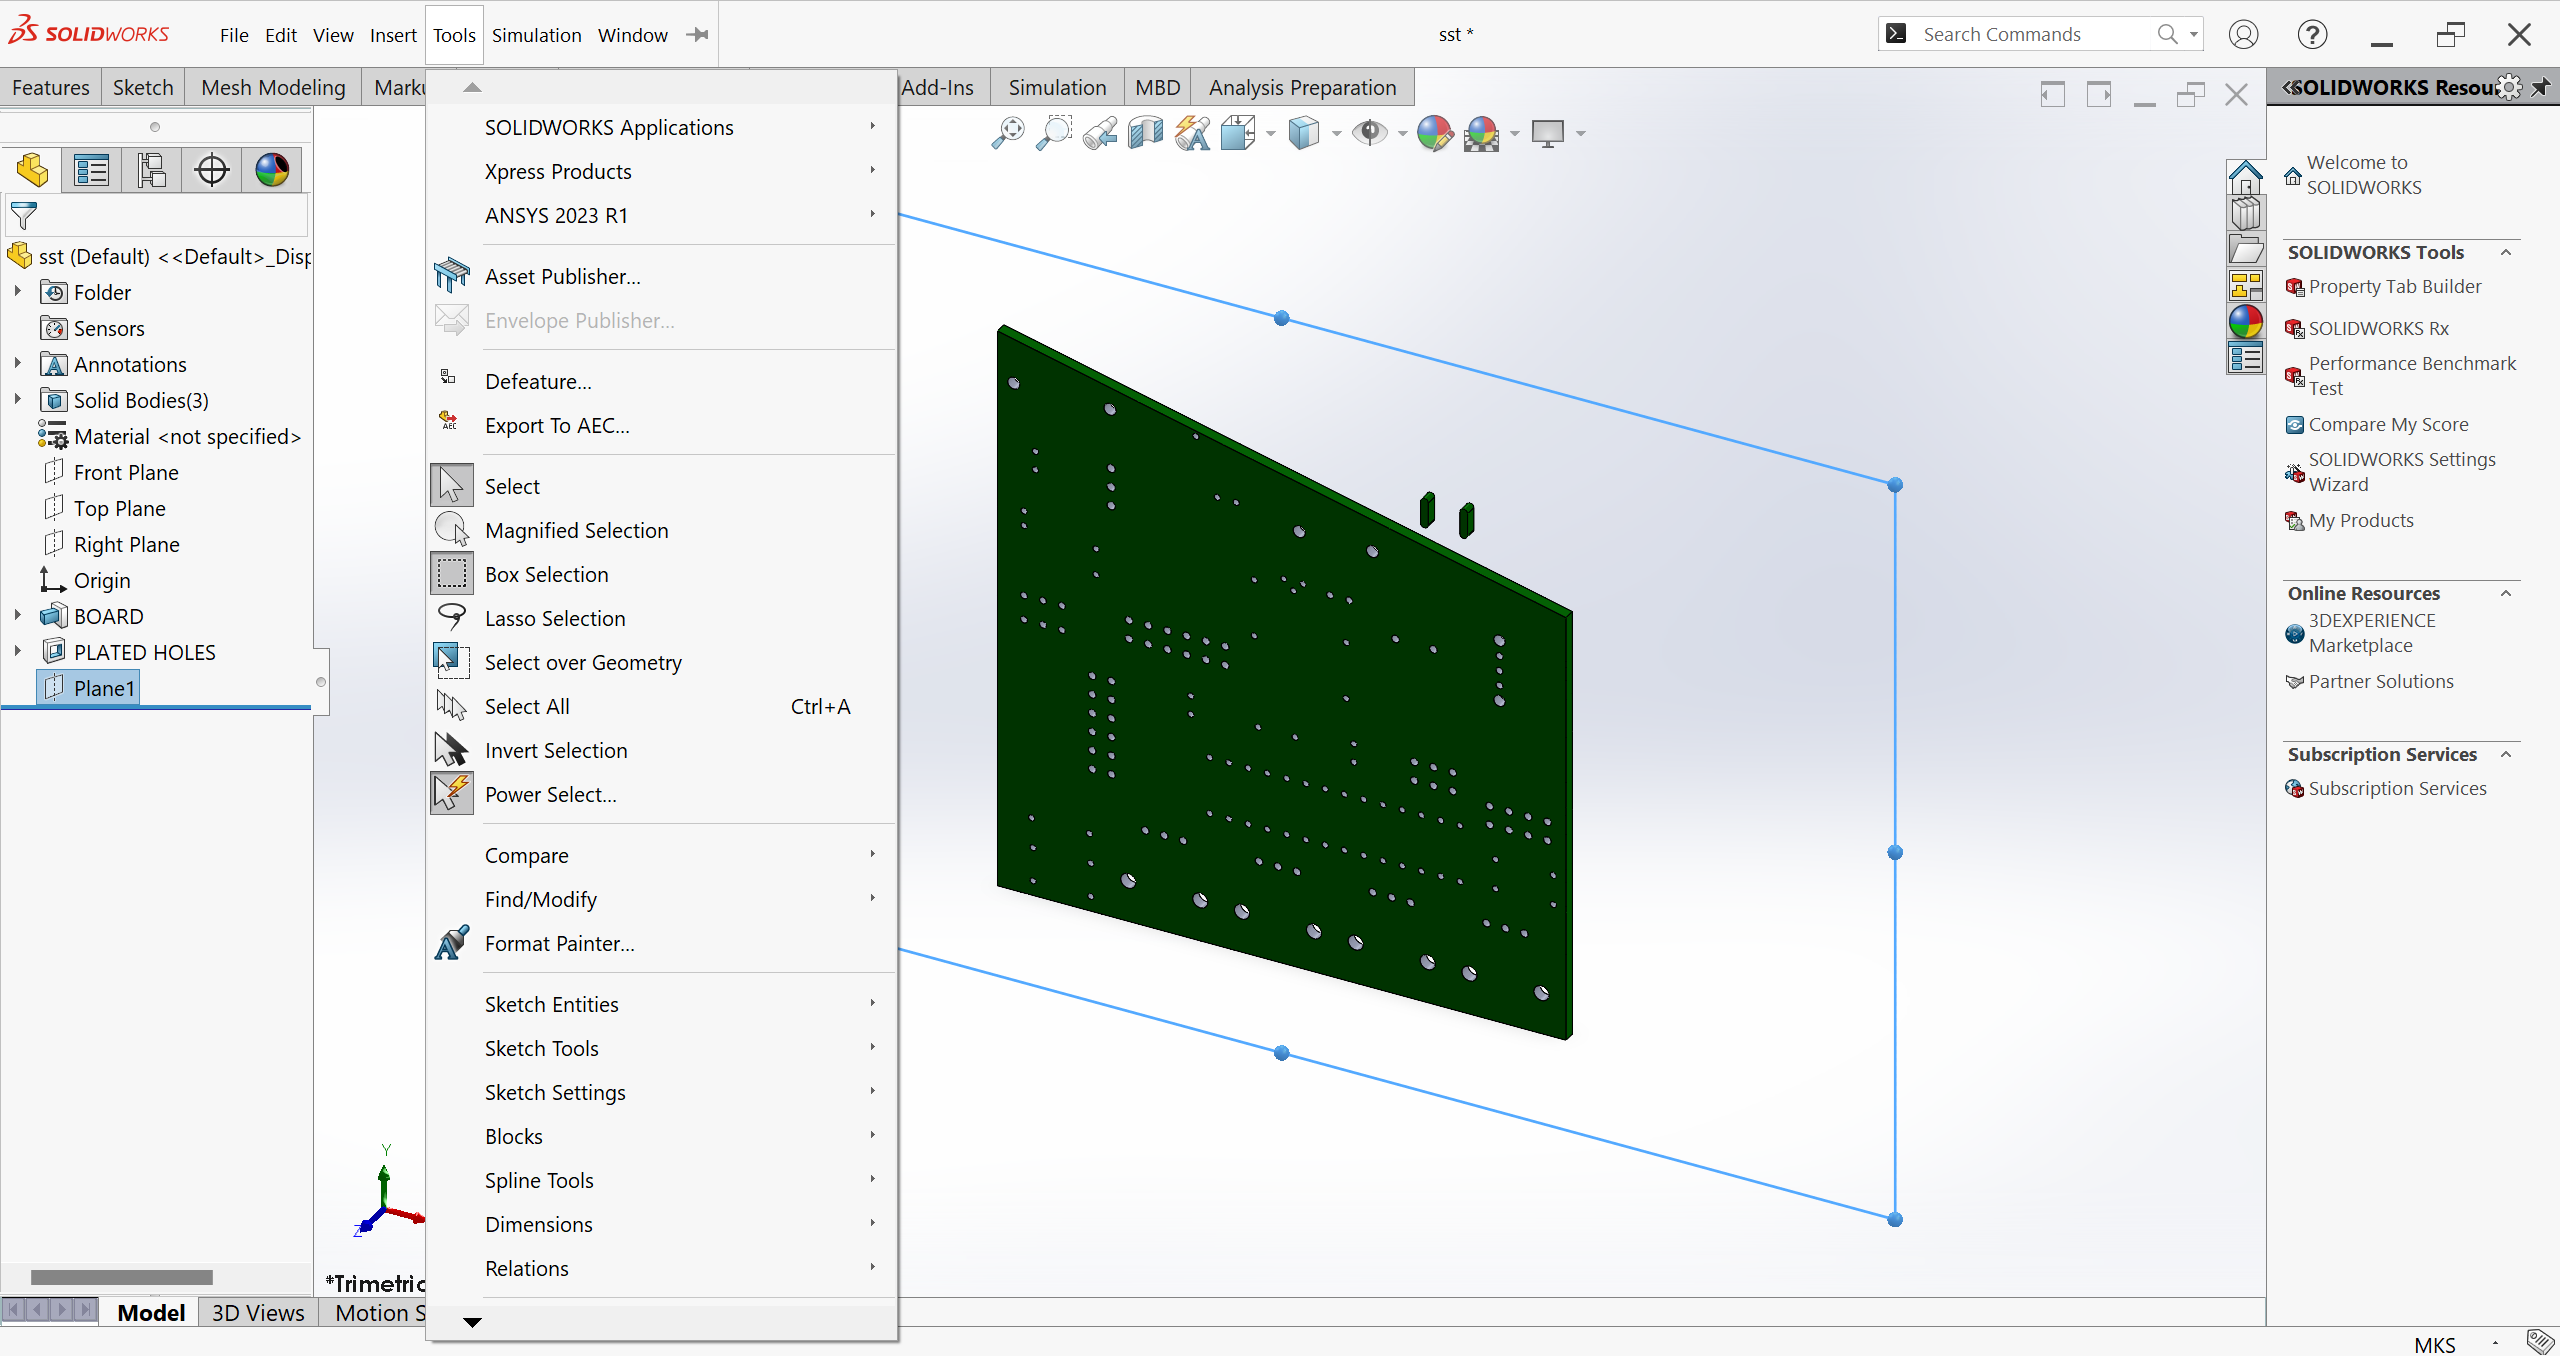
\includegraphics[scale=0.2]{../img/scrot/Screenshot-2024-05-06-175849.png}
  \caption{Скриншот импортированного IDF печатной платы в САПР \textit{SOLIDWORKS}}
\end{figure}

Однако и эта попытка кончилась провалом. Импортированная плата не имела вообще никаких компонентов и была упрощена черезмерно.

Было понятно, что нужно будет переделывать в \textit{Altium Designer} какую-то часть проекта, чтобы получить полноценную трёхмерную модель печатной платы.

Однако совсем не хотелось терять проделанную работу, поэтому было установлено расширение для \textit{Altium Designer} под названием \textit{KiCAD Importer}, которое предоставляло мастер импорта проектов из \textit{KiCAD}.

\begin{figure}[H]
  \centering
  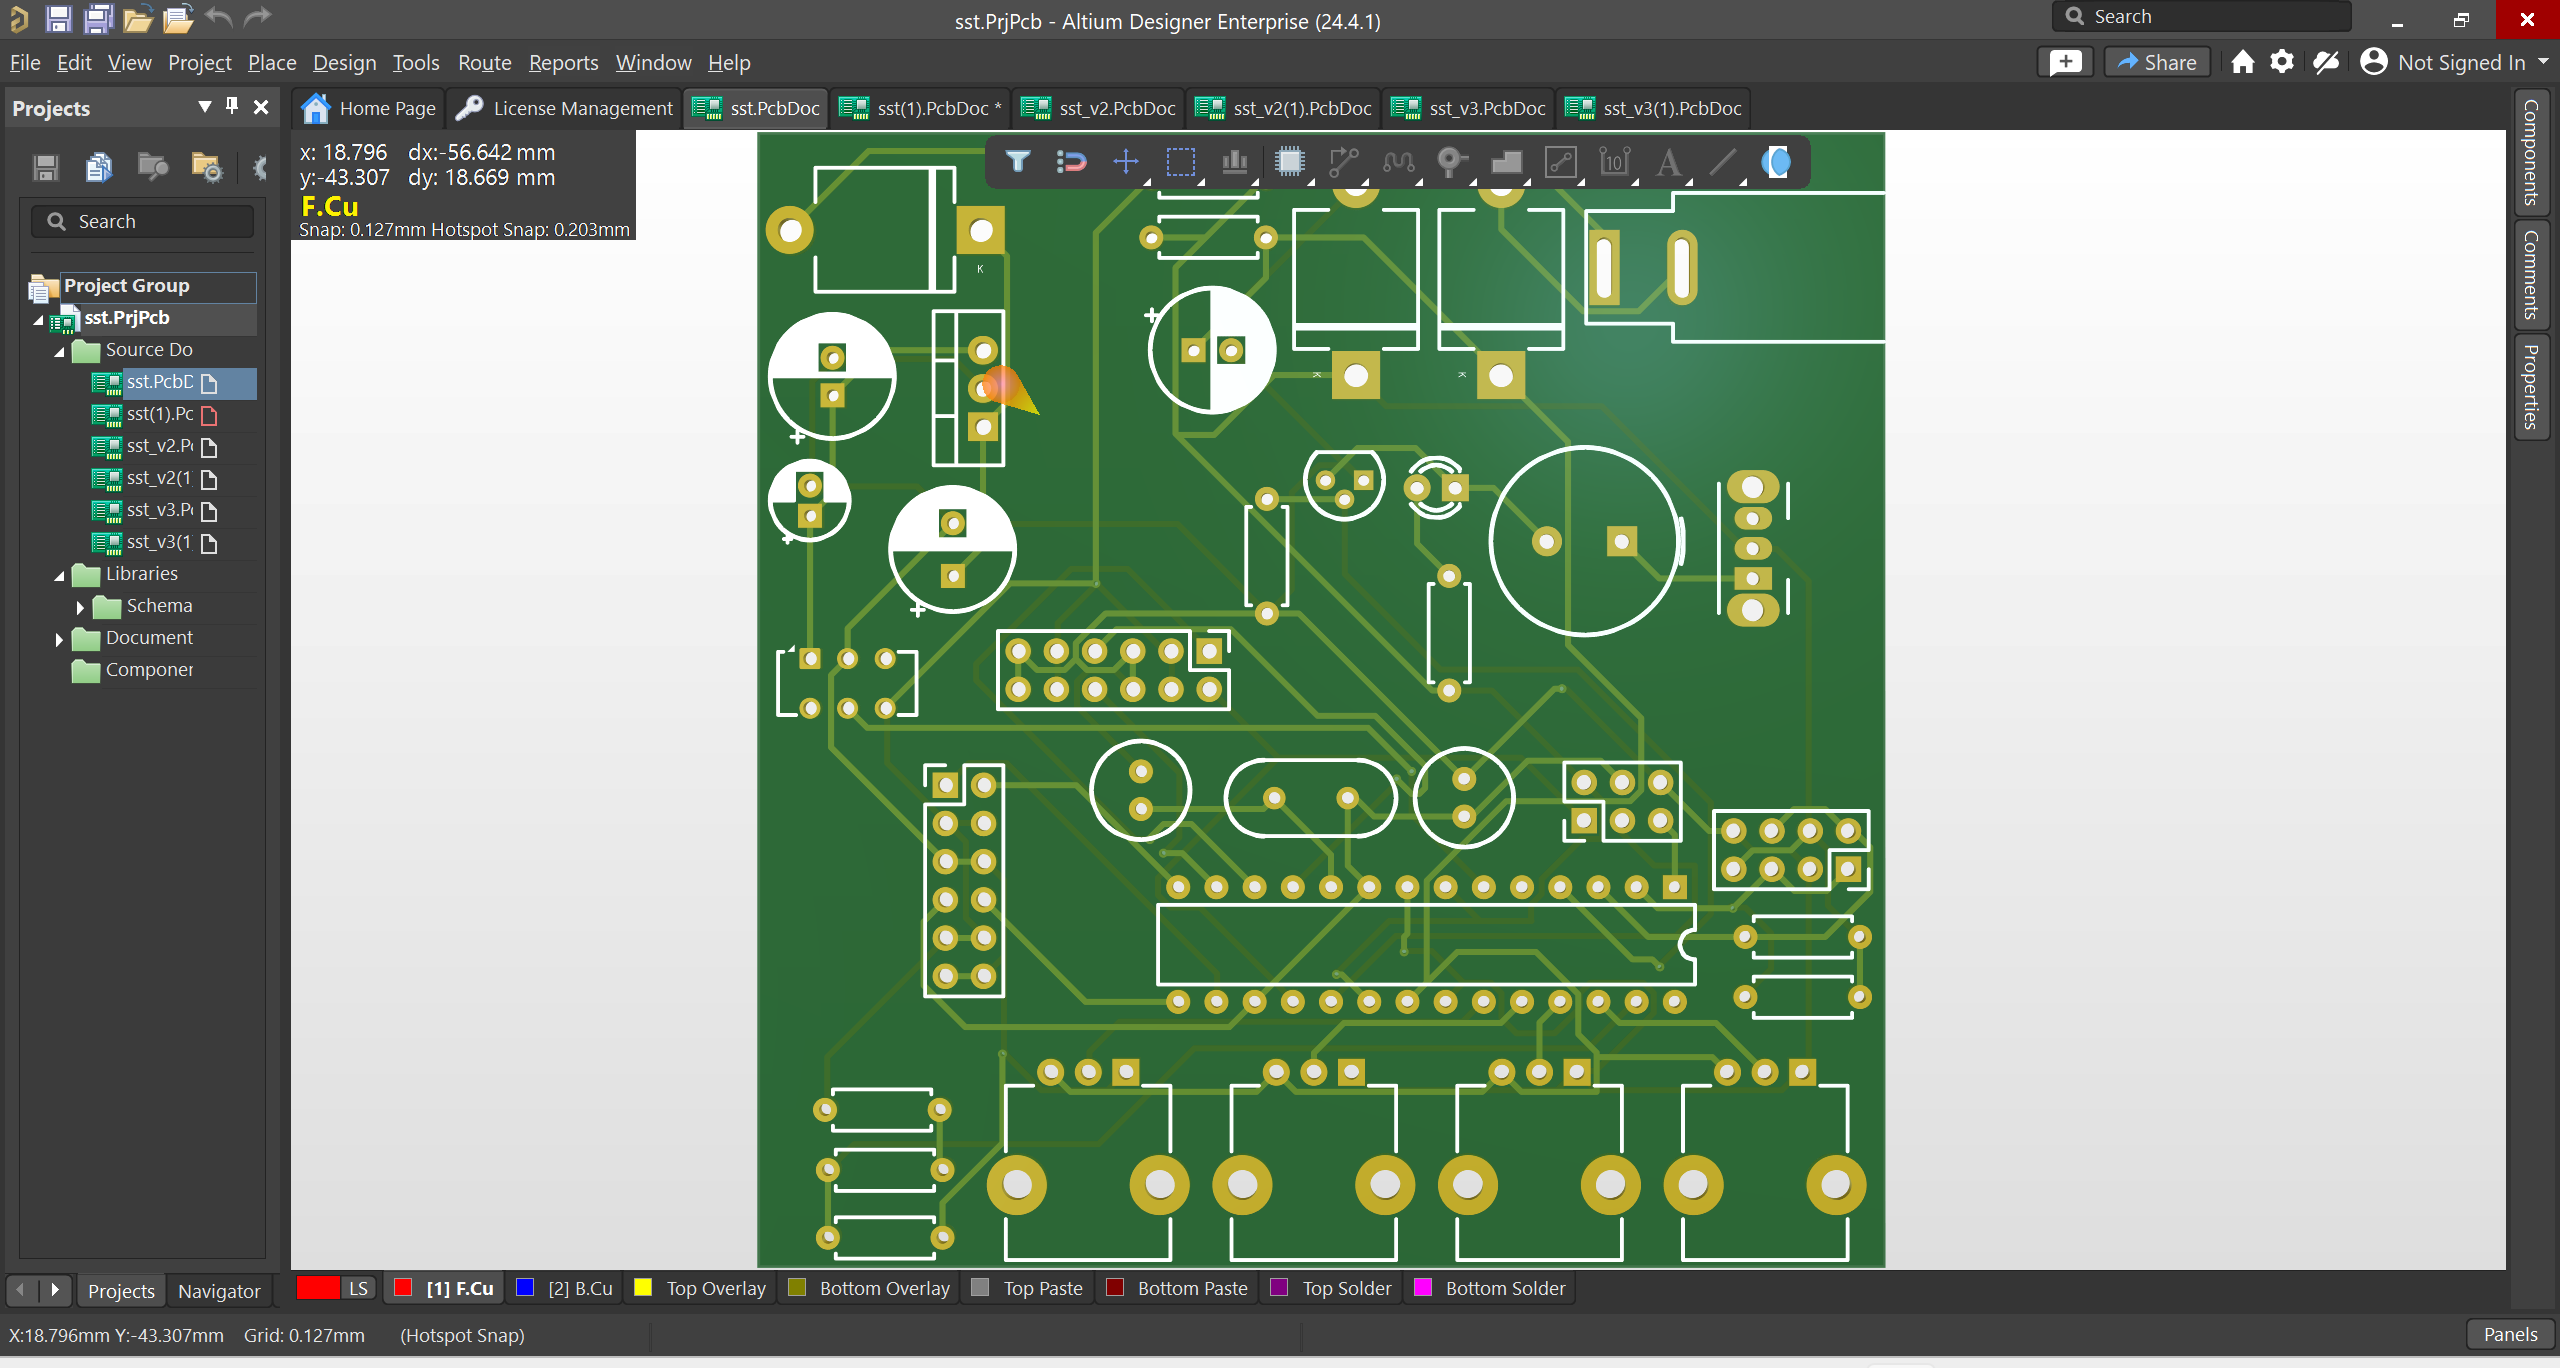
\includegraphics[scale=0.2]{../img/scrot/Screenshot-2024-05-08-110214.png}
  \caption{Скриншот трёхмерной модели имопрированной из \textit{KiCAD} печатной платы в \textit{Altium Designer}}

\end{figure}

В результате импорта в проекте \textit{Altium} появились соотвественно три документа печатных плат.

После этого модели были экспортированы из \textit{Altium} в формате \textit{IDF}. Затем был осуществлен импорт этих моделей в \textit{SOLIDWORKS}. В отличие от моделей получившихся при предыдущей попытке экспорта теперь была сохранена геометрия платы и остались контуры (\textit{Sketch}) от элементов расположенных на ней. В последствии инструментом \textit{Extrude} на вкладке \textit{Analysis Prepartion} было осуществлено выдавливание фигур, схожих по объёму с трехмерным моделями печатных плат.

\begin{figure}[H]
  \centering
  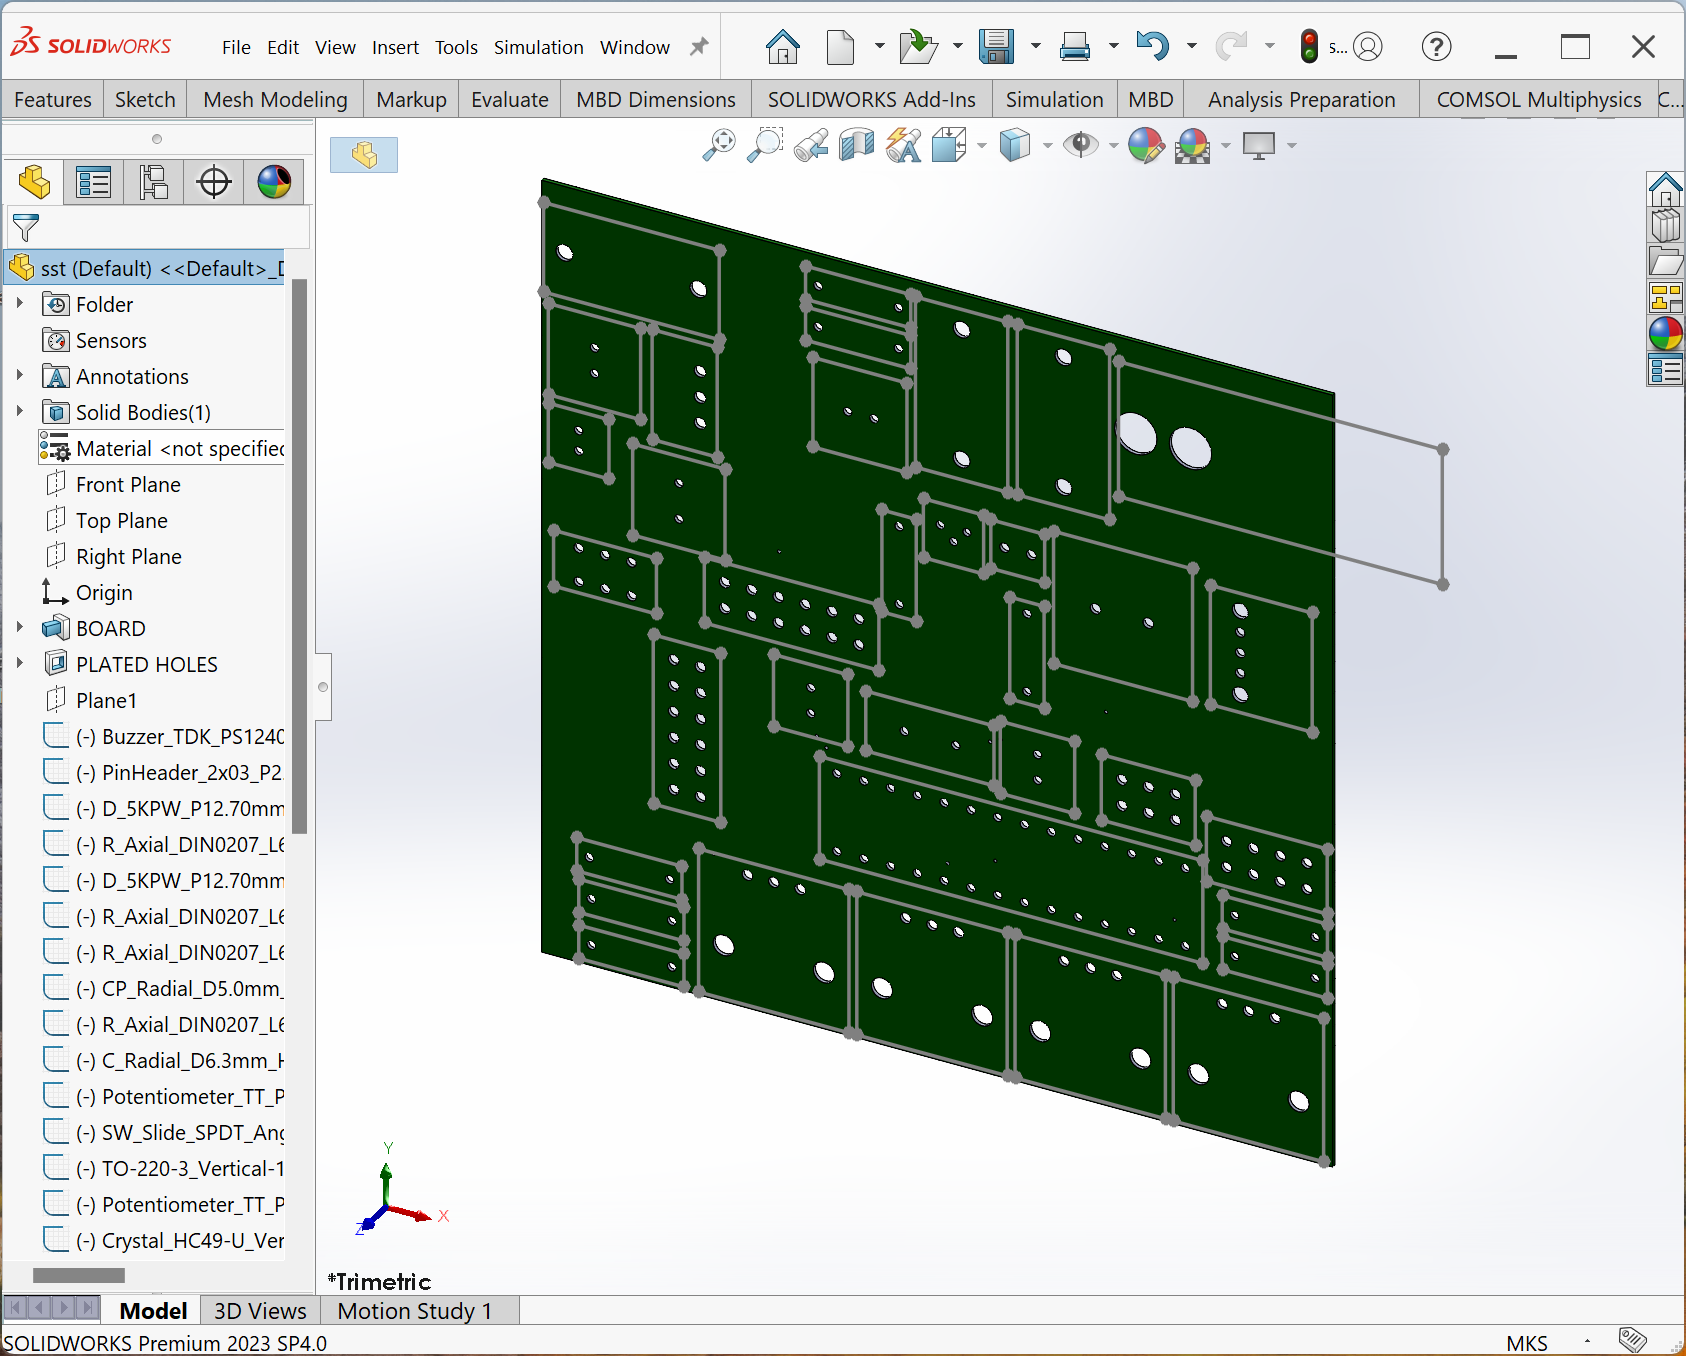
\includegraphics[scale=0.3]{../img/scrot/Screenshot-2024-05-08-132748.png}
  \caption{Скриншот только импортированной в \textit{SOLIDWORKS} печатной платы в формате IDF из \textit{Altium Designer}. Видны контуры посадочных мест.}

\end{figure}


Изначально зная о том, сколько работы будет потрачено, на всего лишь, экспорт трёхмерной модели печатной платы я бы не стал использовать для этого САПР \textit{KiCAD} даже несмотря на возможное удобство в непоредственно проектировании.

Из этого можно сделать вывод, что при выполнение подобных проектов, при выбьоре определенного САПР стоит руководствоваться совместимостью его с другими программами.
Или хотя бы заренее проверять на каком-то миниатюрном проекте-приемере возможность перенесения модели из одной программы в другую.

Что же касается непосредственно проектирвония, то, возможно, было опрометчиво отказываться от использования монтажных отверстий в плате.
